%%%%%%%%%%%%%%%%%%%%%%%%%%%%%%%%%%%%%%%%%
% Short Sectioned Assignment LaTeX Template Version 1.0 (5/5/12)
% This template has been downloaded from: http://www.LaTeXTemplates.com
% Original author:  Frits Wenneker (http://www.howtotex.com)
% License: CC BY-NC-SA 3.0 (http://creativecommons.org/licenses/by-nc-sa/3.0/)
%%%%%%%%%%%%%%%%%%%%%%%%%%%%%%%%%%%%%%%%%

%----------------------------------------------------------------------------------------
%	PACKAGES AND OTHER DOCUMENT CONFIGURATIONS
%----------------------------------------------------------------------------------------

\documentclass[paper=a4, fontsize=11pt]{scrartcl} % A4 paper and 11pt font size

% ---- Entrada y salida de texto -----

\usepackage[T1]{fontenc} % Use 8-bit encoding that has 256 glyphs
\usepackage[utf8]{inputenc}

% ---- Idioma --------

\usepackage[spanish, es-tabla]{babel} % Selecciona el español para palabras introducidas automáticamente, p.ej. "septiembre" en la fecha y especifica que se use la palabra Tabla en vez de Cuadro

% ---- Otros paquetes ----

\usepackage{amsmath,amsfonts,amsthm} % Math packages
\usepackage{graphics,graphicx, floatrow} %para incluir imágenes y notas en las imágenes
\usepackage{graphics,graphicx, float} %para incluir imágenes y colocarlas
\usepackage{hyperref} % url in references
\usepackage{textcomp}
\usepackage{listings}
\usepackage{titlesec}

% Para hacer tablas comlejas
\usepackage{multirow}
\usepackage{threeparttable}

\usepackage{fancyhdr} % Custom headers and footers
\pagestyle{fancyplain} % Makes all pages in the document conform to the custom headers and footers
\fancyhead{} % No page header - if you want one, create it in the same way as the footers below
\fancyfoot[L]{} % Empty left footer
\fancyfoot[C]{} % Empty center footer
\fancyfoot[R]{\thepage} % Page numbering for right footer
\renewcommand{\headrulewidth}{0pt} % Remove header underlines
\renewcommand{\footrulewidth}{0pt} % Remove footer underlines
\setlength{\headheight}{13.6pt} % Customize the height of the header

\numberwithin{equation}{section} % Number equations within sections (i.e. 1.1, 1.2, 2.1, 2.2 instead of 1, 2, 3, 4)
\numberwithin{figure}{section} % Number figures within sections (i.e. 1.1, 1.2, 2.1, 2.2 instead of 1, 2, 3, 4)
\numberwithin{table}{section} % Number tables within sections (i.e. 1.1, 1.2, 2.1, 2.2 instead of 1, 2, 3, 4)

\setlength\parindent{0pt} % Removes all indentation from paragraphs - comment this line for an assignment with lots of text

\newcommand{\horrule}[1]{\rule{\linewidth}{#1}} % Create horizontal rule command with 1 argument of height

\usepackage{textcomp}
\usepackage{listings}

%----------------------------------------------------------------------------------------
%	DATOS
%----------------------------------------------------------------------------------------

\newcommand{\myName}{Francisco Javier Bolívar Lupiáñez}
\newcommand{\myDegree}{Grado en Ingeniería Informática}
\newcommand{\myFaculty}{E. T. S. de Ingenierías Informática y de Telecomunicación}
\newcommand{\myDepartment}{Lenguajes y Sistemas de Información}
\newcommand{\myUniversity}{\protect{Universidad de Granada}}
\newcommand{\myLocation}{Granada}
\newcommand{\myTime}{\today}
\newcommand{\myTitle}{Práctica 1}
\newcommand{\mySubtitle}{Implementación distribuida de un algoritmo paralelo de datos usando MPI}
\newcommand{\mySubject}{Programación Paralela}
\newcommand{\myYear}{2015-2016}

%----------------------------------------------------------------------------------------
%	PORTADA
%----------------------------------------------------------------------------------------


\title{	
	\normalfont \normalsize 
	\textsc{{\bf \mySubject \space (\myYear)} \\ \myDepartment} \\[20pt] % Your university, school and/or department name(s)
	\textsc{\myDegree \\[10pt] \myFaculty \\ \myUniversity} \\[25pt]
	\horrule{0.5pt} \\[0.4cm] % Thin top horizontal rule
	\huge \myTitle: \mySubtitle \\ % The assignment title
	\horrule{2pt} \\[0.5cm] % Thick bottom horizontal rule
	\normalfont \normalsize
}

\author{\myName} % Nombre y apellidos

\date{\myTime} % Incluye la fecha actual
%----------------------------------------------------------------------------------------
%	INDICE
%----------------------------------------------------------------------------------------

\begin{document}

\lstdefinestyle{C} {
	basicstyle=\scriptsize,
	frame=single,
	language=C,
	numbers=left
}
	
\setcounter{page}{0}

\maketitle % Muestra el Título
\thispagestyle{empty}

\newpage %inserta un salto de página

\listoffigures

\newpage

%----------------------------------------------------------------------------------------
%	DOCUMENTO
%----------------------------------------------------------------------------------------

\section{Planteamiento}

En esta práctica se llevará a cabo la paralelización del \textbf{algoritmo Floyd} para la búsqueda del camino más corto en un grafo.
\\ \\
Se desarrollarán dos versiones:
\begin{itemize}
	\item \textbf{Unidimensional}: Se repartirán las filas de la matriz a los procesos.
	\item \textbf{Bidimensional}: Se repartirán submatrices de la matriz a los procesos.
\end{itemize}

\subsection{Algoritmo de Floyd}

El algoritmo de Floyd deriva una matriz en N pasos (tantos como número de nodos), obteniendo en cada paso una matriz intermedia con el camino más corto entre cada par de nodos.

\subsubsection{Pseudocódigo}

\begin{lstlisting}[style=c]
M[i][j] = A
for k = 0 to N-1
  for i = 0 to N-1
    for j = 0 to N-1
      M[i][j] = min(M[i][j], M[i][k] + M[k][j])
\end{lstlisting}

\section{Solución}

\subsection{Versión unidimensional}

\subsubsection{Descripción}

Para solucionarlo con este enfoque, asumiendo que el tamaño del problema es divisible entre el número de procesos, \textbf{cada proceso tendrá una matriz local de tamaño $N/P \times N$}.
\\ \\
\textbf{El reparto se realizará por bloques}. Es decir. Al primer proceso le corresponderán las primeras N/P filas, al segundo las siguientes... Por ejemplo, si el tamaño del problema es 8 y tenemos 4 procesos, al $P_{0}$ le corresponderás las filas 0 y 1, al $P_{1}$ las 2 y 3, al $P_{2}$ las 4 y 5 y al $P_{3}$ las 6 y 7.
\\ \\
En el cálculo de cada submatriz resultado, cada proceso necesitará, en el paso k, la fila k y puede tener suerte y ser suya o no y corresponderle a otro proceso. Entonces debería comunicarse con éste para poder realizar el cálculo. Por tanto, en cada iteración del primer bucle k, \textbf{el proceso detectará si la fila k le pertenece y si es así, hace un \textit{broadcast} al resto de procesos}.
\\ \\
Por tanto, para solucionar el problema, nos basta con un \textbf{\textit{scatter} para repartir la matriz}, un \textbf{\textit{broadcast} para difundir cada fila k} y un \textbf{\textit{gather} para recolectar la matriz resultado} y el único problema que nos podríamos encontrar es el traducir de local a global un índice según lo que se necesite.

\subsubsection{Pseudocódigo}

\begin{lstlisting}[style=c]
M[i][j] = A
for k = 0 to N-1
  broadcast(K)
  for i = 0 to N/P-1
    for j = 0 to N-1
      M[i][j] = min(M[i][j], M[i][k] + K[j])
\end{lstlisting}

\subsubsection{Problemas y soluciones}

El principal problema que se puede encontrar en esta versión es, como he comentado anteriormente, el \textbf{traducir un índice de local en un proceso a global}.
\\ \\
No obstante, si se trabaja con índices locales, es decir, el búcle va desde 0 a N/P, solo se necesita el índice global para comprobar que no se está iterando sobre la diagonal de la matriz (i=j, i=k o j=k).
\\ \\
El otro problema con el que me encontré fue durante el \textit{broadcast} de la fila k. Y es que al escribir la sentencia \texttt{MPI\_BCast} no cambié el índice del proceso raíz y siempre mandaba la fila k el proceso 0. Esto es fácil de corregir, una vez detectado el fallo, pues el índice del proceso raíz siempre será k / tamaño de bloque (siendo el tamaño de bloque N/P).

\subsubsection{Código}

\lstinputlisting[style=c]{src/floyd1D.cpp}

\subsection{Versión bidimensional}

\subsubsection{Descripción}

Para solucionarlo con este enfoque, asumiendo que el tamaño del problema es divisible entre la raíz cuadrada del número de procesos, \textbf{cada proceso tendrá una matriz local de tamaño $N/\sqrt{P} \times N/\sqrt{P}$}.
\\ \\
El reparto, a diferencia del enfoque anterior, no es inmediato. En la versión unidimensional realizábamos un \textit{scatter} directamente porque se repartían celdas consecutivas en memoria. En este caso, al distribuir submatrices cuadradas, \textbf{deberemos definir un tipo de dato MPI}.
\\ \\
Se realizarán $\sqrt{P}$ particiones en cada dimensión, obteniendo P submatrices de tamaño $N/\sqrt{P} \times N/\sqrt{P}$ cada una. Se repartirán a los procesos de izquierda a derecha y arriba abajo. Si, por ejemplo, tuviésemos 9 procesos, la de arriba a la izquierda le correspondería al $P_{0}$, la de arriba al centro al $P_{1}$, la de arriba a la derecha al $P_{2}$, la del centro a la izquierda al $P_{3}$, la del centro al $P_{4}$, la del centro a la derecha al $P_{5}$, la de abajo a la izquierda al $P_{6}$, la de abajo al centro al $P_{7}$ y la de abajo a la derecha al $P_{8}$.
\\ \\
Si para el reparto y recolección del resultado se complica la cosa, para el cálculo de éste también. Y es que antes, con la repartición unidimensional, tan solo se necesitaba la fila k, pero \textbf{ahora se necesitan valores en las dos dimensiones para calcular el resultado}: hace falta una subfila k y una subcolumna k de los procesos que están colocados en la misma columna y fila respectivamente.
\\ \\
Para llevar a cabo estas comunicaciones hará falta definir \textbf{dos comunicadores} y asignarlos a cada proceso para que, en el comunicador horizontal se comuniquen aquellos que se encuentran en la misma fila y en el vertical los que están en la misma columna.

\subsubsection{Pseudocódigo}

\begin{lstlisting}[style=c]
M[i][j] = A
for k = 0 to N-1
  broadcast(filK)
  broadcast(colK)
  for i = 0 to N/sqrt(P)-1
    for j = 0 to N/sqrt(P)-1
      M[i][j] = min(M[i][j], ColK[i] + FilK[j])
\end{lstlisting}

\subsubsection{Problemas y soluciones}

La complicación de la implementación de esta versión, como ya se comentaron, son el trabajar un \textbf{tipo de dato MPI personalizado} y con \textbf{comunicadores para filas y columnas}.
\\ \\
Para trabajar con un tipo de dato personalizado, hay que definirlo y empaquetarlo para poder hacer tanto el \textit{scatter} como el \textit{gather}.
\\ \\
\textbf{Se define con \texttt{MPI\_Tipe\_vector}} y se le pasa el número de grupos de bloque (en nuestro caso, las filas de la submatriz), el número de elementos de cada bloque (columnas de la submatriz), la separación entre un bloque y otro (tamaño del problema), el tipo de dato (entero) y el nombre del tipo de dato MPI que se usará. Una vez definido, se realiza un \texttt{MPI\_Type\_commit}.
\\ \\
A continuación hay que \textbf{empaquetarlos en un búfer de envío}, para eso se realizarán tantas iteraciones en un bucle como número de procesos haya. En cada una de estas iteraciones se tiene que empaquetar con \texttt{MPI\_Pack} a la que se le pasarán como parámentros el puntero al inicio del búfer de entrada (para ello se debe calcular el desplazamiento desde el inicio de la matriz para cada proceso), el número de datos de entrada (en nuestro caso 1), el tipo de dato (que será el que definimos anteriormente), el puntero al búfer de salida, el tamaño de éste, la posición (que inicializamos a 0 y el propio \texttt{MPI\_Pack} se encarga de modificar) y el comunicador. De entre todas estas variables, la única que habría que calcular es el desplazamiento desde el inicio de la matriz para apuntar al inicio de cada submatriz y sería:
\[ desplazamiento = col_P \times tama_{bloque} + fil_P \times tama_{bloque}^{2} \times \sqrt{P} \]
donde:
\[ col_P = i / \sqrt{P} \]
\[ fil_P = i \% \sqrt{P} \]
\[ tama_{bloque} = N / \sqrt{P} \]
\\ \\
Una vez empaquetado se puede realizar el \textit{scatter} con los siguientes parámetros: El búfer de entrada sería el búfer de envío que usamos como búfer de salida en el \texttt{MPI\_Pack}, el tamaño el necesario para almacenar los enteros de la submatriz, el tipo de dato \texttt{MPI\_PACKED}, el búfer de recepción el puntero a la submatriz local, el tamaño el de la submatriz, el tipo de dato entero, el proceso raíz el 0 (que ha sido el que ha realizado todas las operaciones anteriores de definición y empaquetado del tipo de dato) y el comunicador el global.

\subsubsection{Código}

\lstinputlisting[style=c]{src/floyd2D.cpp}

\section{Resultados}

\begin{tabular}{ | c | c c c | c c | }
	\hline
	N		&	$ T_{sec} $	&	$ T_{1D} $	&	$ T_{2D} $	 &	$ S_{1D} $	 &	$ S_{2D} $	\\
	\hline
	64      &	0,000396482 &	0,000868711 &	0,0008886901 &	0,4564023343 &	0,4461414615	\\
	128     &	0,003013494 &	0,004452289 &	0,004570981  &	0,6768415078 &	0,6592663588	\\
	256     &	0,0234622   &	0,02117407  &	0,023623352  &	1,1080628335 &	0,9931782755	\\
	512     &	0,2003635   &	0,10693829  &	0,11696271   &	1,8736366553 &	1,7130545282	\\
	1024    &	1,403187    &	0,4415758   &	0,4668597    &	3,1776809327 &	3,0055860465	\\
	\hline
\end{tabular}
\captionof{table}{Tiempos y ganancia para P = 4 y N = 64, 128, 256, 512 y 1024}

\begin{figure}[H]
	\centering
	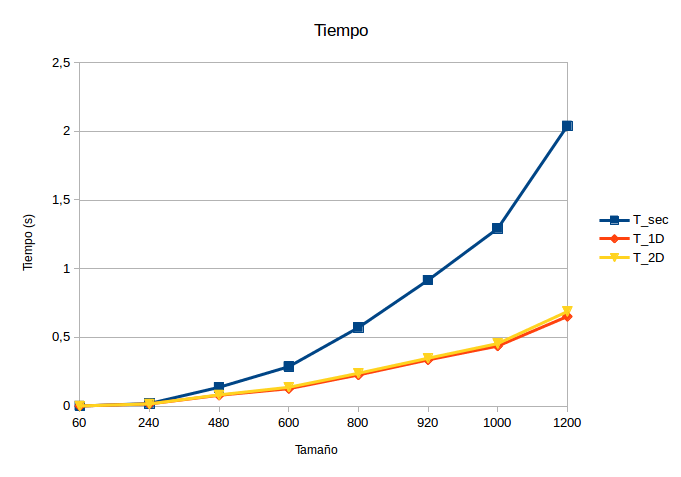
\includegraphics[width=9cm]{img/tiempo}
	\caption{Gráfica de tiempo para P = 4 y N = 64, 128, 256, 512 y 1024}
	\label{fig:grafica_tiempo}
\end{figure}

\begin{figure}[H]
	\centering
	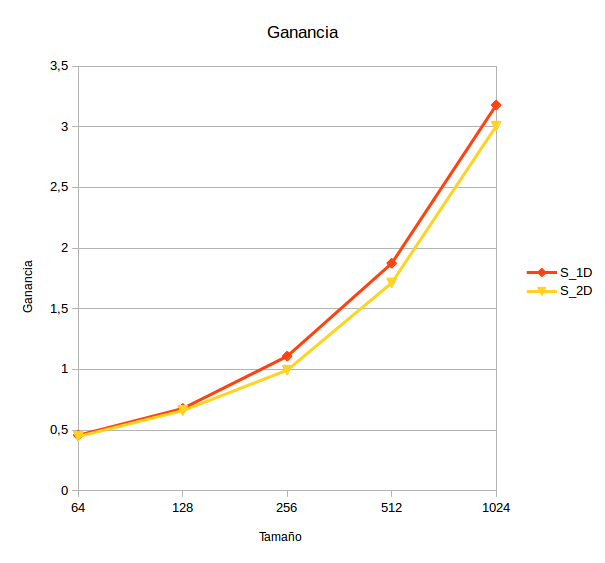
\includegraphics[width=9cm]{img/ganancia}
	\caption{Gráfica de ganancia para P = 4 y N = 64, 128, 256, 512 y 1024}
	\label{fig:grafica_ganancia}
\end{figure}

\end{document}